\documentclass[
headings=optiontohead,              %allows double headers
12pt,                               %fontsize 
DIV=13,                             %koma script diveider amount. tells koma how much of the site can be written to
open=right,                         %starting page on twosided texts 
toc=bibliographynumbered            %bibliography gets a number and is listed in the table of contents
]{scrreport}
\raggedbottom
\setlength{\parindent}{0em}

\usepackage[utf8]{inputenc}                     %correct encoding of output, technically not needed anymore
\usepackage[T1]{fontenc}                        %correct encoding of output, technically not needed anymore
\usepackage[ngerman, english]{babel}             %font that supports English
\usepackage{upgreek}                            %non-cursive Greek letters
\usepackage[stretch=10,shrink=10,protrusion=true,expansion=true,final]{microtype}                          %prettier blocksatz
\usepackage{hyperref}                           %links for everything
\usepackage{color}                              %allows for setting in different colors
\usepackage[autooneside=false,automark]{scrlayer-scrpage}%page-style with "Kolumnentitel" (title of current chapter is displayed at the top)
\usepackage[autostyle=true]{csquotes}           %context-sensitive-quotes -> quotation marks that are set correctly for the context
%\usepackage{lmodern}                           %alternative font (better use libertinus)
\usepackage[sb]{libertinus}                     %use the font libertinus (needs to be installed from the web)
\usepackage[slantedGreek]{libertinust1math}     %math mode improvement for libertinus
\usepackage{siunitx}                            %physical units setting
\usepackage{icomma}                             %commas in lists get extra space if needed                        
\usepackage{amsfonts,amssymb,amstext,amsmath,amsthm} %better math mode (\mathrm and \text) and symbols
\usepackage{xspace}                             %works to improve own commands and provides "\xspace"-command, that puts a space if needed
\usepackage{ifthen}                             %more control over non-obligatory parameters
\usepackage[onehalfspacing]{setspace}           %control the spacing between lines and in enumeration lists
\usepackage[backend=biber, style=phys, url=true, biblabel=brackets]{biblatex}         %citations with "modern" backend and an physics-accepted citation style
%\usepackage{graphicx}                           %work with graphics 
\usepackage{pdfpages}                           %allows including of pdfs into this pdf
\usepackage{booktabs}                           %better table formatting
\usepackage{multicol}                           %allows for the definition of multi-columns in tables
\usepackage{multirow}                           %allows for the definition of multirow-tables instead of just multicolumn
\usepackage{arydshln}                           % allows dotted hline
\setlength\dashlinedash{1.5pt}
\setlength\dashlinegap{0pt}
\setlength\arrayrulewidth{0.3pt}
\usepackage{tikz}                               %generate nice svg-pictures directly in latex
\usepackage{quantikz}
\usepackage[siunitx,european,straightvoltages, oldvoltagedirection]{circuitikz}
\usetikzlibrary{babel}
\usepackage{url}                                %sometimes needed by biblatex, technically no longer needed

\usepackage{todonotes}                          %adds todonotes (added by Jan Wozniak)
\usepackage{placeins} %for \FloatBarrier 
%\clubpenalty10000                                   % Schusterjunge, orphan
%\widowpenalty10000                                  % Hurenkind, Witwe
%\displaywidowpenalty=10000                          % Make document obey stricter rules considering "schusterjungen" and "hurenkinder"
\renewcommand{\topfraction}{0.8}                    % allows for more chilled "text to image ratio" 
\renewcommand{\bottomfraction}{0.8}
\renewcommand{\textfraction}{0.1}
\renewcommand{\floatpagefraction}{0.8}

% \renewcaptionname{ngerman}{\figurename}{Abb.}       %"Abbildung" becomes "Abb." in German
%\setcapindent{0cm}                                 %useful if image captions have multiple lines. Removers indentation below "Abb."
%\setlength{\parindent}{0cm}                         %removes indentation at start of new paragraphs


%bibliography slots are redefined/modified here
\DeclareFieldFormat{journaltitle}{\textsl{#1}\isdot}
\DeclareFieldFormat{titlecase}{{#1}}


%COLORS
\definecolor{dblue}{rgb}{0,0,0.5}
\definecolor{dred}{rgb}{0.5,0,0}
\definecolor{dgrey}{rgb}{0.5,0.5,0.5}

%overwrite the coma-script definitions
\addtokomafont{pagehead}{\normalfont\color{dgrey}}                  %overwrite the coma-script definitions
\addtokomafont{sectioning}{\rmfamily\color{black}\boldmath}         %rmfamily puts headings in "normal" "Serifenschrift" instead of "sans-serif"  boldmath ensures a bold math font in subscripts
\addtokomafont{captionlabel}{\bfseries\footnotesize}                %better Abb. format
\addtokomafont{caption}{\footnotesize}                          

%! hyphenation commonly used words can be spelled here to provide latex with the correct places to make linebreaks
                                  %another file that holds format information
%! Commands by Jan Geiger and Jonas Kell 
\usetikzlibrary{shapes.misc}
\tikzset{cross/.style={cross out, draw=black, minimum size=2*(#1-\pgflinewidth), inner sep=0pt, outer sep=0pt}, cross/.default={1pt}}

\newcommand*{\fullref}[1]{\hyperref[{#1}]{\textit{\ref*{#1} \nameref*{#1}}}}
\newcommand*{\fullpage}[1]{\hyperref[{#1}]{Seite \pageref*{#1}}}
\newcommand*{\fullpages}[1]{\hyperref[{#1}]{Seiten \pageref*{#1}ff}}
\newcommand*{\kapref}[1]{\hyperref[{#1}]{{Kapitel \ref*{#1}}}}

\renewcommand*{\arraystretch}{1.5}

\newcommand{\dx}[1]{\; \text{d}#1}
\newcommand{\da}[1]{\text{d}#1}
\newcommand{\rot}{\text{rot }}
\newcommand{\grad}{\text{grad }}
\renewcommand{\div}{\text{div }}

\newcommand{\kb}{k_\text{B}}

\newcommand{\myexp}[1]{\ensuremath{\exp\left\{#1\right\}}}
\newcommand{\myln}[1]{\ensuremath{\ln\left(#1\right)}}
\newcommand{\mylog}[1]{\ensuremath{\log\left(#1\right)}}
\newcommand{\mycoth}[1]{\ensuremath{\coth\left(#1\right)}}
\newcommand{\mydet}[1]{\ensuremath{\det\left(#1\right)}}
\newcommand{\mytr}[1]{\ensuremath{\text{Tr}\left(#1\right)}}

\newcommand{\mysin}[1]{\ensuremath{\sin\left(#1\right)}}
\newcommand{\mycos}[1]{\ensuremath{\cos\left(#1\right)}}
\newcommand{\mytan}[1]{\ensuremath{\tan\left(#1\right)}}




\newcommand{\abs}[1]{\ensuremath{\left|#1\right|}\xspace}
\newcommand{\smallabs}[1]{\ensuremath{\big|#1\big|}\xspace}


\newcommand{\norm}[1]{\ensuremath{||#1||}\xspace}

\newcommand{\sigmax}[1][]{\ensuremath{\hat{\sigma}_{\text{x} \ifthenelse{\equal{#1}{}}{}{, {#1}}}}\xspace}
\newcommand{\sigmay}[1][]{\ensuremath{\hat{\sigma}_{\text{y} \ifthenelse{\equal{#1}{}}{}{, {#1}}}}\xspace}
\newcommand{\sigmaz}[1][]{\ensuremath{\hat{\sigma}_{\text{z} \ifthenelse{\equal{#1}{}}{}{, {#1}}}}\xspace}




                                %another file that holds predefined commands

\graphicspath{{./Grafiken/}}              %custom paths for folders in that graphics can be found

% \linespread{1.1}                        %line-spacing can be controlled here

\usetikzlibrary{calc}                   %calculations inside tikz
\usetikzlibrary{arrows}                 %better arrows for tikz
\usepackage{pgfplots}                   %better plotting with tikz
\pgfplotsset{compat=1.16}               %better plotting with tikz
\pgfkeys{/pgf/number format/.cd, use comma}


\sisetup                                %setup for siunitx
{
detect-all,
range-units = brackets,                 %better display of error ranges
per-mode=symbol-or-fraction,            %more dynamic frac usage in inline/displaymath mode
separate-uncertainty,                   %for better +- , \pm when including an error range 
}

\hypersetup
{
hidelinks,
colorlinks=true,
linkcolor=dblue,            %deep blue linkcolor
urlcolor=dblue,             %deep blue linkcolor
citecolor=dblue,            %deep blue linkcolor
pdfauthor = {Jan Wozinak, Jan Geiger, Emiliano Godinez},                                   %write details into the expanded file properties
pdftitle = {FP32},  
pdfkeywords = {Fortgeschrittenen-Praktikum},            
pdfsubject = {FP32}
}


\AtBeginDocument{
	\let\mathbb\relax
	\DeclareMathAlphabet\PazoBB{U}{fplmbb}{m}{n}
	\newcommand{\mathbb}{\PazoBB}
}


\addbibresource{literatur.bib}              %initialize bibtex with correct file


%!START THE DOCUMENT

\begin{document}
    \thispagestyle{empty}           %make sure title page ist not numbered or anything else
    
\newcommand{\getTitle}{FOPRA 34: Simulating Quantum Many-Body Dynamics on a Current Digital Quantum Computer}
\newcommand{\getAuthor}{Franz von Silva Tarouca}
\newcommand{\getAuthorI}{Christian Gnandt}
\newcommand{\getAuthorII}{Cristian Emiliano Godinez}

\newcommand{\getSupervisor}{Johannes Feldmeier}
\newcommand{\getSupervisorI}{Wilhelm Kadow}
\newcommand{\getSupervisorII}{Yujie Liu}


\begin{titlepage}
    \centering

    \IfFileExists{logos/tum.pdf}{%
        
\includegraphics[height=20mm]{logos/tum.pdf}
    }{%
        \vspace*{20mm}
    }

    \vspace{5mm}
    {\huge\MakeUppercase{Department of Physics}}\\

    \vspace{5mm}
    {\large\MakeUppercase{Technische Universität München}}\\

    \vspace{20mm}
    % {\Large Fortgeschrittenenpraktikum (FOPRA)}

    \vspace{15mm}
    {\huge\bfseries \getTitle{}}

    \vspace{20mm}
    \begin{tabular}{l l}
        Authors:          & \getAuthor{} \\
                          & \getAuthorI{} \\
                          & \getAuthorII{} \\
        Supervisors:      & \getSupervisor{} \\
                          & \getSupervisorI{} \\
                          & \getSupervisorII{} \\
        Submission Date: & \today{} \\
    \end{tabular}

    \IfFileExists{logos/faculty.pdf}{%
        \vfill{}
        
\includegraphics[height=20mm]{logos/faculty.pdf}
        % \hspace{20mm}
        % \includegraphics[height=20mm]{logos/wsi_icon_med_transp.png}
    }{}
\end{titlepage}           %include title-page
    \cleardoublepage                %make sure, that if double-page is active, to reset the double page counter
    \pagestyle{scrheadings}         %puts current chapters title into the header in small grey font
    \pagenumbering{roman}           %number the pages of the table of contents in roman numerals
    \tableofcontents

\newpage   %table of contents include
    \pagenumbering{arabic}          %number the pages of the main document in Arabic numerals
    \clearpairofpagestyles
    \ihead{\leftmark}
    \ohead{\Ifstr{\leftmark}{\rightmark}{}{\rightmark}}
    \cfoot*{\pagemark}


    \cleardoublepage
    

    \chapter{Introduction}
    The field of quantum many-body physics covers a wide range of systems with increasing scale, with many relying on numerical simulations to solve their equations. Quantum computing devices are an ideal platform to explore these open questions, as they are able to naturally handle the exponential complexity of a quantum system. This report studies dynamical phase transitions, a quantum many-body phenomena, in a specific Ising model using simulations with the Google Cirq framwork for noisy intermediate scale quantum computing. The code uses common methods in quantum simulation, such as Trotterization, Generalized Amplitude Damping channel and Tomography, to run a local simulation that mirrors the protocol used to control and compute on a real quantum device. The theoretical groundwork and coding tasks are taken from a manual \cite{manual}. The report summarizes some of the core theoretical concepts needed for the exercises and discusses the results of the simulations.

    \chapter{Numerical Methods}
    \section{Matrix Product States (MPS)}


Within a given Hilbert Space, a random state follows a volume law.
In other words, the entanglement entropy of this state grows linearly with the "volume".
For a one-dimensional system the "volume" corresponds to the length of the system. \\

On the other hand, the ground states of a gapped Hamiltonian obey an area law, i.e. the entropy is proportional to the area of the cut that partitions the Hilbert Space.
For a 1D case this implies that the entropy is constant with respect to the increase of the system size $N$. \\

For the random states mentioned previously, the entanglement entropy is close to its maximum value, for which the Schmidt coefficients are close to being constant.
In contrast, the states following an area law (like a ground state) are slightly entangled, which results in most of the weight being distributed in only a few Schmidt coefficients.
This subtle but important observation allows for the introduction of a compressed representation of these "product states" known as: 
matrix-product states (MPS).\\

We consider a one dimensional chain made up of $N$ sites, with each individual site $n$ having a local basis labeled as $\ket{j_n}$ for $j_n = 0, \dots, d$, where $d$ is the dimension of the n$^{th}$ site's Hilbert Space.
The figure below shows a diagrammatic representation of a tensor with $N$ physical legs.

\begin{figure}[h!]
    \centering
    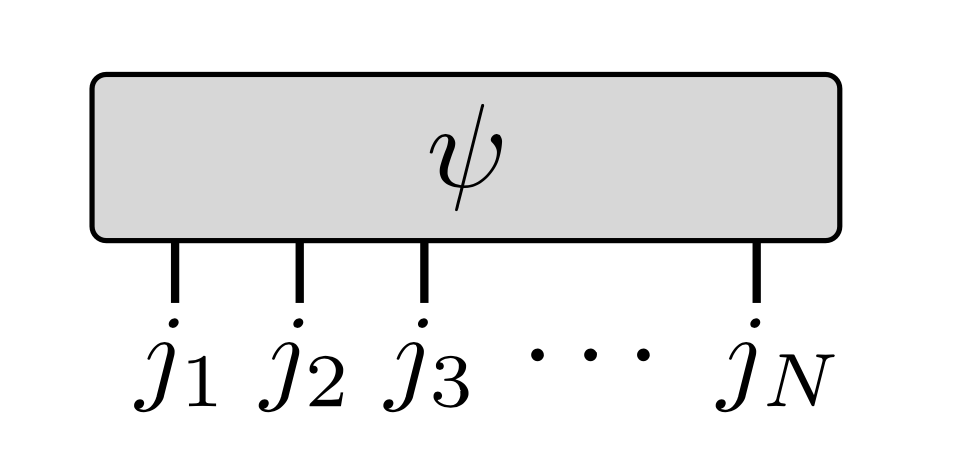
\includegraphics[scale=0.5]{Figures/MPS_1.png}
    \caption{Diagram representation of a $N$ dimensional tensor. Source: \cite{anleitung}}
    \label{fig:mps-1}
\end{figure}

The problem is that even for relatively simple configurations, such as a half spin system, an exact simulation is possible only up to approximately 40 sites \cite{anleitung} due to the exponentially increasing number of entries to store.
This is exactly why MPS representation comes in handy.
A general pure state can be written in MPS as~\cite{anleitung}:

\begin{equation}
    \ket{\Psi} = \sum_{j_1,...,j_N} M^{[1]j_1} M^{[2]j_2} ... M^{[N]j_N} \ket{j_1,j_2,...,j_N}
    \label{eq:MPS_1}
\end{equation}

Where each $ M^{[n]j_n}$ is a $\chi_n \times \chi_{n+1}$ dimensional matrix and $[n]$ tells us that, for a general state, the matrices on each site could be different.
In order to obtain a number as the result of the matrix multiplication, the convention is that $\chi_1 = \chi_{N+1} = 1$, meaning that the first and last matrices are actually vectors.\\

From the superscript $j_n$ we see that there are $d$ matrices corresponding to each site, and these can be grouped to form a 3-degree tensor as shown here:

\begin{figure}[h!]
    \centering
    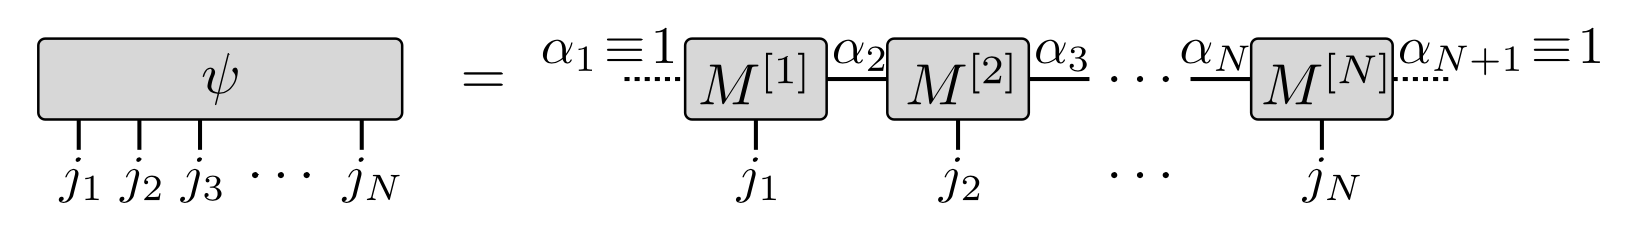
\includegraphics[scale=0.5]{Figures/MPS_2.png}
    \caption{MPS representation of quantum state. Source \cite{anleitung}}
    \label{fig:mps-2}
\end{figure}

Where $\alpha_i$ are the virtual legs or bonds, which are by nature different than the physical indices $j_n$\\

A so called "canonical form" can be defined based on the freedom of choice of the matrices representing our quantum state. This results in the equation \cite{anleitung}:

\begin{equation}
    \ket{\Psi} = \sum_{j_1,...,j_N} \Lambda^{[1]} \Gamma^{[1]j_1}\Lambda^{[2]} \Gamma^{[2]j_2}\Lambda^{[3]}...\Lambda^{[N]} \Gamma^{[N]j_N} \Lambda^{[N+1]} \ket{j_1,j_2,...,j_N}
    \label{eq:mps-canonical}
\end{equation}

Where the matrices $\Lambda^{[n+1]}$ are square diagonal matrices that contain the Schmidt values $\Lambda^{[n+1]}_{\alpha_{n+1}}$ in the diagonal and the $\Gamma^{[n]j_n}$ are such that $\Gamma^{[n]j_n}\Lambda^{[n+1]}$ for each site returns the original state.
This grouping, however, can also be done in two different standard ways:
\begin{equation}
    A^{[n]j_n} = \Lambda^{[n]} \Gamma^{[n]j_n}
    \label{eq:mps-left-canonical}
\end{equation}
\begin{equation}
    B^{[n]j_n} = \Gamma^{[n]j_n}\Lambda^{[n+1]}
    \label{eq:mps-right-canonical}
\end{equation}

A state represented solely using matrices of the form given in equation \ref{eq:mps-left-canonical} is known as \textbf{left canonical form}, while one using only matrices of the form in \ref{eq:mps-right-canonical} is known as \textbf{right canonical form}.
Mixed representations are also possible.\\

With this representation, calculating expectation values (of local operators) becomes a relatively easy task. It is useful also to realize that converting from left to right representation (and vice versa) can be readily accomplished by multiplying by the corresponding inverse of the matrix $\Lambda$.

\section{Time Evolving Block Decimation (TEBD)}

The time evolving block decimation (TEBD) algorithm allows to calculate the time evolution of a state in MPS representation.
This can be done both with a real or imaginary time evolution.
The latter can be employed to calculate the ground state using the following relation from \cite{anleitung}:

\begin{equation}
    \ket{\psi_{GS}} = \lim_{\tau \rightarrow \infty} \frac{e^{-\tau H}\ket{\psi_0}}{||e^{-\tau H}\ket{\psi_0}||}
    \label{eq:tebd-gs}
\end{equation}    

\textbf{Note:}\\
With the help of Trotterization, the time evolution operator can be applied to a state in MPS representation in order to perform a local transformation efficiently.
Since local unitaries do not affect the entanglement, the $\Lambda$ values do not change and thus the amount of information remains the same.
This, however, is not the case for two site unitaries like the ones present in our Ising Hamiltonian. 
Due to this, a cutoff in the Schmidt coefficients ought to be implemented to avoid an exponential grow of information stored.

\section{Dynamic Structure Factor}

The dynamic structure provides information about the excited states of the system under study.
In moment and frequency space the dynamic structure for the system of our interest is defined as in \cite{anleitung}:

\begin{equation}
    S^{\alpha\alpha}(k,\omega) = \frac{1}{2\pi} \sum_\mathcal{R} e^{-i k\cdot \mathcal{R}} \int_{-\infty}^{\infty} e^{i\omega t} \langle \mathcal{\hat{O}^{\alpha \dagger}_{\mathcal{R}}}(t) \mathcal{\hat{O}}^{\alpha}_0(0) \rangle
\end{equation}

To obtain the value of the dynamic structure $S^{\alpha\alpha}$ numerically, it is necessary to discretize the integral (i.e. approximate it by a finite sum) and to allow the time evolution to occur only for a finite time $T$.
The latter results in the lost of information about low frequencies corresponding to small excitations. \\

In addition, considering only a finite time is equivalent to convoluting the real signal with a square window which results in Gibbs oscillations showing up in the numerical results of $S^{\alpha \alpha}$.
To prevent this oscillations from affecting our results, the time series under the Fourier Transform can be convoluted with a Gaussian window function, resulting in the smoothening of the edges and thus avoiding undesired oscillations. 



    \chapter{Day 1 -- Basics of Matrix Product States}
    \section{Readout Matrix Unfolding}
Current and near-term quantum computing devices are subject to significant inaccuracies due to the multitudes of noise sources affecting the computation and the measurement process. With appropriate error mitigation, however, these noisy intermediate-scale quantum (NISQ) devices can still be utilized. Readout matrix unfolding is such an error mitigation protocol that combats readout errors. The protocol consists of a calibration and an unfolding sequence. Here we are considering an $n$ qubit device. The calibration is measuring the readout matrix $P$ that quantifies the measurement errors. The element $P_{ab}$ is the probability that the bitstring $b$ is measured after preparing the bitstring $a$. The matrix thus has $2^n\times2^n$ entries. For small errors rates we approximate the relation between a measured arbitrary bitstring $v'$ and the error-free bitstring $v$ as
\begin{equation}
    v_a' = \sum_b P_{ab}v_b .
    \label{eq:readout_matrix}
\end{equation}
The error mitigated result $v$ is obtained by inverting the readout matrix $P$ from the calibration and applying it to the measured bitstring $v'$. If the measurement is normalized before this procedure, then the mitigated result is still normalized and thus physical in that aspect. This is shown by looking at the absolute value of the sum over $a$ in equation \eqref{eq:readout_matrix}. The probabilistic definition of $P$ demands that all possible outcomes, here the columns, sum to unity, $\sum_a P_{ab} = 1$.
\subsubsection{Exercise 1}
\begin{equation}
        \abs{\sum_a v_a'} = \abs{\sum_{a,b}P_{ab}v_b} = \abs{\sum_b v_b} = 1
\end{equation}
While normalization is therefore guaranteed for an appropriate input, the final result $v$ might still be nonphysical, as negative entries are possible. For this report this method with an additional check against negatives values will be sufficient.
\section{Quantum Teleportation}
Quantum teleportation is a protocol to copy a quantum state $\ket{\varphi}$ over any distance between 2 locations. The sender and receiver need to share an entangled EPR qubit pair and the original state is destroyed in the process. The protocol involves preparing and measuring qubits in the EPR basis, seen in equation \eqref{eq:epr}.
\begin{equation}
    \ket{\Phi^\pm} = \frac{1}{\sqrt{2}}\left(\ket{00} \pm \ket{11}\right) \quad
    \ket{\Psi^\pm}  = \frac{1}{\sqrt{2}}\left(\ket{01} \pm \ket{10}\right)
    \label{eq:epr}
\end{equation}
\subsubsection{Exercise 2}
The preparation starting from the ground state $\ket{00}$ is achieved by creating a superposition with the Hadamard gate H and then entangling them with the CNOT gate. Figure \ref{fig:prepare_EPR} shows the circuits to create each EPR state.
\begin{figure}[h]
    \centering
    \begin{subfigure}[t]{0.19\textwidth}
        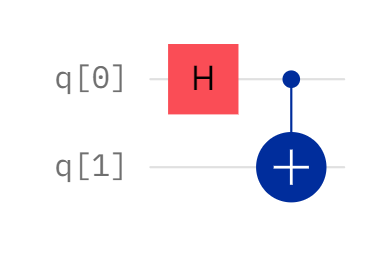
\includegraphics[width=\textwidth]{tex/figures/exercise02_01.png}
        \caption{$\ket{\Phi^+} = \frac{1}{\sqrt{2}}(\ket{00} + \ket{11}$}
        \label{fig:e0201}
    \end{subfigure}
    \begin{subfigure}[t]{0.24\textwidth}
        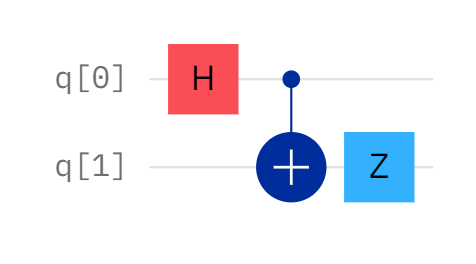
\includegraphics[width=\textwidth]{tex/figures/exercise02_02.png}
        \caption{$\ket{\Phi^-} = \frac{1}{\sqrt{2}}(\ket{00} - \ket{11}$}
        \label{fig:e0202}
    \end{subfigure}
    \begin{subfigure}[t]{0.24\textwidth}
        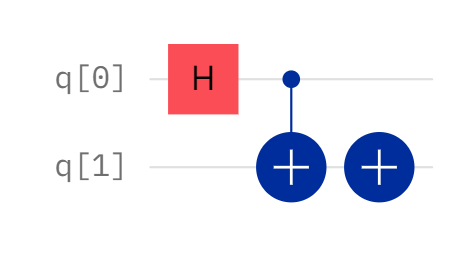
\includegraphics[width=\textwidth]{tex/figures/exercise02_03.png}
        \caption{$\ket{\Psi^+} = \frac{1}{\sqrt{2}}(\ket{01} + \ket{10}$}
        \label{fig:e0203}
    \end{subfigure}
    \begin{subfigure}[t]{0.29\textwidth}
        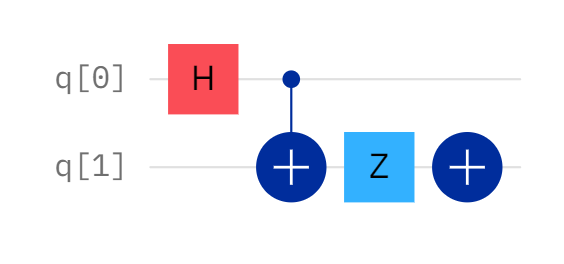
\includegraphics[width=\textwidth]{tex/figures/exercise02_04.png}
        \caption{$\ket{\Psi^-} = \frac{1}{\sqrt{2}}(\ket{01} - \ket{10}$}
        \label{fig:e0204}
    \end{subfigure}
    \caption{Preparation circuit for all EPR states. The plus symbol denotes addition modulo 2 and therefore an X or NOT gate.}
    \label{fig:prepare_EPR}
    \addtocounter{figure}{-1}
\end{figure}
To measure in the EPR basis, the gate to create $\ket{\Phi^+}$ is applied in reverse before the qubits are measured sequentially in the computational basis. The mapping between the computational basis and the EPR basis is determined by the circuit. With circuit \ref{fig:e0201} the mapping is $\ket{\Phi^+} \leftrightarrow \ket{00}$, $\ket{\Phi^-} \leftrightarrow \ket{10}$, $\ket{\Psi^+} \leftrightarrow \ket{01}$ and $\ket{\Psi^-} \leftrightarrow \ket{11}$.
\subsubsection{Exercise 3}
Depending on the outcome of the EPR measurement, a controlled unitary needs to be applied to obtain the exact original state. This is clear when the complete system state, including the original state $\ket{\varphi} = \alpha\ket{0} + \beta\ket{1}$, is rewritten in the EPR basis
\begin{equation}
\begin{aligned}
    \label{eq:decomposition}
    \ket{\varphi}_0\frac{1}{\sqrt{2}}\left(\ket{00}_{12} + \ket{11}_{12}\right) &= \ket{\Phi^+}_{01}\left(\alpha\ket{0}_2 + \beta\ket{1}_2\right) + \ket{\Phi^-}_{01}\left(\alpha\ket{0}_2 - \beta\ket{1}_2\right) \\
    &+ \ket{\Psi^+}_{01}\left(\alpha\ket{1}_2 + \beta\ket{0}_2\right)
    + \ket{\Psi^-}_{01}\left(\alpha\ket{1}_2 - \beta\ket{0}_2\right).
\end{aligned}
\end{equation}
The state of qubit q[2] after the EPR measurement will carry the $\alpha$ and $\beta$ coefficients of the original q[0] state, however, sometimes swapped or with an additional sign. The sign is removed with a controlled Z gate (CZ), the switch reversed with a controlled X gate (CX).
\begin{figure}
    \centering
    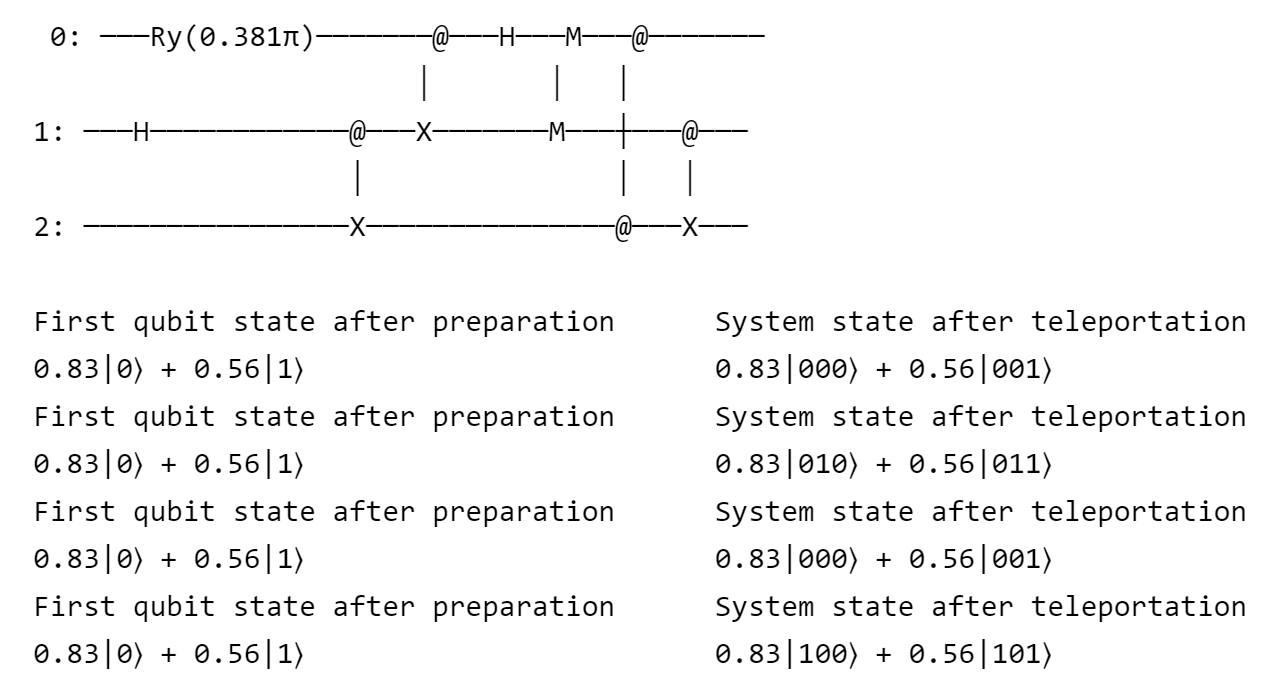
\includegraphics[width=0.8\linewidth]{tex/figures/exercise04.png}
    \caption{Circuit diagram and output for quantum teleportation. The state $\ket{\varphi}$ is initially on qubit 0 and is then copied to qubit 2. The @ symbol denotes the control qubit in a controlled gate. M shows measurements on qubits. The log shows the original and teleported state for four trials.}
    \label{fig:teleportation}
\end{figure}

\subsubsection{Exercise 4}
The complete quantum teleportation protocol is implemented and tested in the Google Cirq framework with the circuit seen in diagram \ref{fig:teleportation}. The corresponding code for all the exercises of Day 1 are found in the appendix chapter \ref{app:day1}, here we will focus on the discussion of the results. The original state $\ket{\varphi}$ is created by rotating around the y axis with a random angle, the example above uses $0.381\pi$. The log included in \ref{fig:teleportation} shows the $\alpha$ and $\beta$ values of $\ket{\varphi}$ after the rotation and the complete system state after teleportation for 4 different trials. The circuit is working correctly as qubit 2 has matching $\alpha$ and $\beta$ values in all trials, independent of the measurement results on qubit 0 and 1. In trial one and three the EPR measurement yielded $\ket{\Phi^+}$, in trial two the $\ket{\Phi^-}$ and in trial three the $\ket{\Psi^+}$ state.

\section{Rabi Oscillation}
Rabi osciallation is the primary phenomena to manipulate single qubits to any desired state. For a two-level system (TLS) quantified along the $\sigmaz$ axis, an oscillating $\sigmax$ component in the Hamiltonian
\begin{equation}
    H = -\frac{\omega_0}{2}\sigmaz + \omega_1\cos(\omega t)\sigmax
\end{equation}
will result in the system oscillating between the ground and excited state $\ket{0}$ and $\ket{1}$.  With the initial state $\ket{\Psi} = \alpha (t)\ket{0} + \beta (t)\ket{1} = \ket{0}$ the dynamics in the rotating wave approximation (RWA) are given by
\begin{equation}
\begin{aligned}
    \label{eq:dynamics}
    \alpha (t) &= e^{-i\omega t/2}\left(\cos \left(\frac{\Omega t}{2}\right) - \frac{i\Delta}{\Omega}\sin \left(\frac{\Omega t}{2}\right)\right), \\
    \beta (t) &= e^{i\omega t/2}\left(-\frac{i\omega_1}{\Omega}\sin \left(\frac{\Omega t}{2}\right)\right)
\end{aligned}
\end{equation}
where $\Delta = \omega - \omega_1$ is the detuning and $\Omega = \sqrt{\omega^2_1 + \Delta^2}$ the Rabi frequency. The condition for RWA to work well is a comparatively weak drive and a small detuning.
\begin{equation}
    \label{eq:conditions}
    \omega_1 \ll \omega_0 \quad \mathrm{and} \quad \Delta \ll 2\omega_0.
\end{equation}
\subsubsection{Exercise 5}
The population of the groud and excited states are retrieved from equations \eqref{eq:dynamics} by taking the square of the absolute value.
\begin{align}
    p_0 &= \abs{\alpha(t)}^2 = \cos^2 \frac{\Omega}{2}t + \left(\frac{\delta}{\Omega}\right)^2\sin^2\frac{\Omega t}{2}
    \label{eq:population0}
\end{align}
\begin{align}
    p_1 &= \abs{\beta (t)}^2  = \left(\frac{\omega_1}{\Omega}\right)^2\sin^2\frac{\Omega t}{2} = \left(\frac{\omega_1}{\Omega}\right)^2\frac{1}{2}\left(1-\cos\Omega t\right)
    \label{eq:population1}
\end{align}
A common method to simulate the dynamics of quantum system with a known Hamiltonian is trotterization. The relevant time interval is discretized into sufficiently small steps and the precise time evolution $U(t)$ is approximated by repeatedly applying a gate that replaces the dynamics for one time step
\begin{equation}
    U(t) = \exp\left(-i\int_0^tH(t)dt\right) \approx \prod^{N-1}_{n=0}\exp\left(-iH(n\delta t)\delta(t)\right).
    \label{eq:trotterization}
\end{equation}
\subsubsection{Exercise 6}
To test the performance of this approximation we simulate Rabi oscillations using trotterization and compare the final state with the analytical values from equation \eqref{eq:population1}. For plot \ref{fig:exercise06_01} and \ref{fig:exercise06_02} the qubit frequency is set to $\omega_0 = 25$, the driving frequency to $\omega_1 = 25.5$ with a driving strength $\omega = 2$. The frequencies are given without units as this is how they are used in the code. What is relevant for their physical properties are their values relative to each other and the considered time range. Qubit and drive are almost in resonance here with only a slight detuning $\Delta = 0.5$, meaning the Rabi frequency $\Omega = 2.062$ is very close to the driving frequency $\omega_1$ and the amplitude $\left(\frac{\omega_1}{\Omega}\right)^2$ is close to 1. This is validated by the plot \ref{fig:exercise06_01} which shows the population of the excited state undergoing a full Rabi oscillation at close to maximum amplitude. The population over the detuning seen in \ref{fig:exercise06_02} also confirms the correct timing for the simulation. At the fixed time $t = \frac{\pi}{\omega_1}$ the interaction equals a $\pi$-pulse that excites the TLS if the detuning $\Delta$ is close to zero, which is clearly visible in the plot.
\begin{figure}[h]
    \centering
    \caption{Comparison between analytical and trotterized calculations of population $\abs{\beta}^2$ for a driven two-level system. The time step for trotterization is $\delta t = 0.05$.}
    \label{fig:exercise06}
    \addtocounter{figure}{-1}
    \begin{subfigure}[t]{0.48\textwidth}
        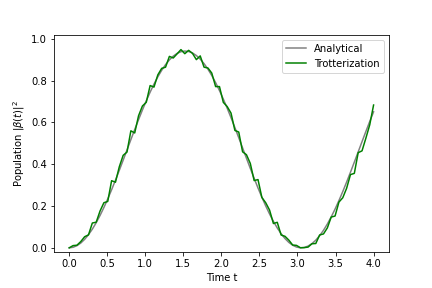
\includegraphics[width=\textwidth]{tex/figures/exercise06_01.png}
        \caption{Population $\abs{\beta}^2$ over time $t$. Rabi oscillation is clearly visible and trotterization works well. Parameters are $\omega_0 = 25, \omega_1 = 25.5$ and $\omega = 2$, resulting in the oscillation period $T = 3.047$.}
        \label{fig:exercise06_01}
    \end{subfigure}
    \begin{subfigure}[t]{0.48\textwidth}
        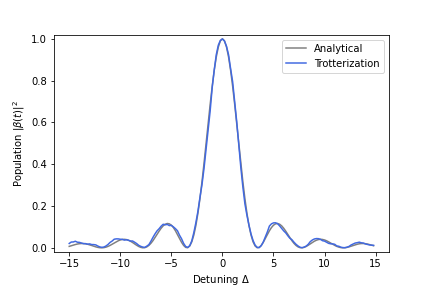
\includegraphics[width=\textwidth]{tex/figures/exercise06_02.png}
        \caption{Population $\abs{\beta}^2$ over detuning $\Delta$ at fixed time $t = \frac{\pi}{\omega_1}$. Parameters are $\omega_0 = 25, \omega_1 = 25.5$ and $\omega \in [10, 40]$ with stepsize $\delta\omega = 0.2$. The $\pi$ pulse fully excites the qubit on resonance.}
        \label{fig:exercise06_02}
    \end{subfigure}
    \\
    \begin{subfigure}[t]{0.48\textwidth}
        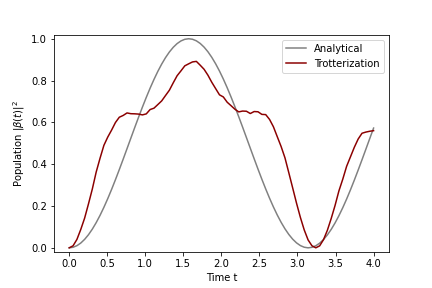
\includegraphics[width=\textwidth]{tex/figures/exercise06_03.png}
        \caption{Population $\abs{\beta}^2$ over time $t$ with $\omega_0 = \omega_1 = \omega = 2$. The driving strength is comparable to the qubit frequency, violating the conditions of the RWA. Trotterization results are more accurate here.}
        \label{fig:exercise06_03}
    \end{subfigure}
    \begin{subfigure}[t]{0.48\textwidth}
        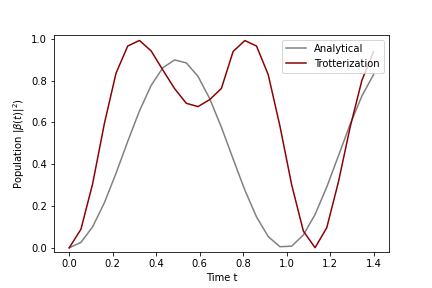
\includegraphics[width=\textwidth]{tex/figures/exercise06_04.png}
        \caption{Population $\abs{\beta}^2$ over time $t$ with $\omega_0, \omega_1, \omega = 3, 1, 6$. Calculations are not in agreement. The detuning and driving strength are larger than qubit frequency, violating all conditions of the RWA.}
        \label{fig:exercise06_04}
    \end{subfigure}
\end{figure}
\\
For the population plots seen in \ref{fig:exercise06_03} and \ref{fig:exercise06_04} the frequencies have been adjusted to $\omega_0 = \omega_1 = \omega$ and $\omega_0 = 3, \omega_1 = 1, \omega = 6$ respectively. In both cases the trotterization and analytical results yield signficantly different results. The discrepancy is explained by the applicability of the RWA used to derive the analytical equations. The driving strength $\omega_1 = 2$ in scenario \ref{fig:exercise06_03} is comparable in size to the TLS frequency $\omega_0 \sim \omega_1$. The system is therefore not in a weak driving regime and RWA is not a good solution. In scenario \ref{fig:exercise06_04} the detuning $\Delta = 3$ has been increased to be close to the TLS frequency $\Delta \sim \omega_0$. Here the parameters violate both conditions for RWA \eqref{eq:conditions} and magnify the difference between the computations.
\subsubsection{Exercise 7}
To get closer to the behavior of physical quantum devices, we extend the simulator with a noise model. These models add the decoherence effects from a physical environment of a quantum computer without simulating the environment itself. We are implementing the generalized amplitude damping channel (GAD) that describes spontaneous emission and thermal excitations. The Kraus operators of the channel are
\begin{align*}
    E_0 &= \sqrt{p}
    \begin{pmatrix}
        1 & 0 \\
        0 & \sqrt{1 - \gamma}
    \end{pmatrix}
    , \quad E_1 = \sqrt{p}
    \begin{pmatrix}
        0 & \sqrt{\gamma} \\
        0 & 0
    \end{pmatrix}
    \\ E_2 & = \sqrt{1-p}
    \begin{pmatrix}
        \sqrt{1-\gamma} & 0 \\
        0 & 1
    \end{pmatrix}
    , \quad E_3 = \sqrt{1-p}
    \begin{pmatrix}
        0 & 0 \\
        \sqrt{\gamma} & 0
    \end{pmatrix}
\end{align*}
with $1-p$ being the probability for thermal excitation and $\gamma$ the probability for spontaneous emission. The channel $\Lambda$ is then with standard definition
\begin{equation}
    \Lambda(\rho) = \sum^3_{i=0} E_i \rho E^\dagger_i .
\end{equation}
\begin{figure}[h]
    \centering
    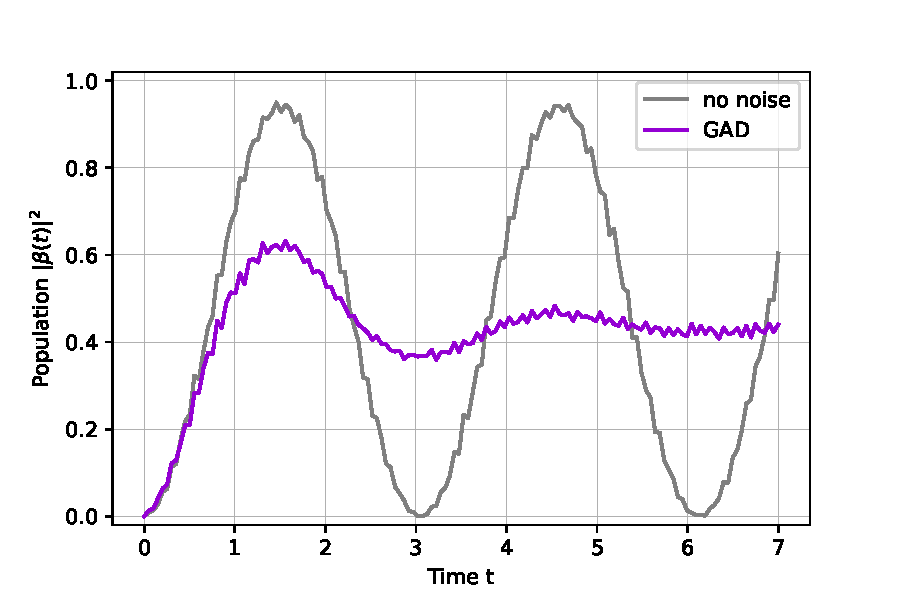
\includegraphics[width=0.7\linewidth]{tex/figures/exercise07_01.pdf}
    \caption{Comparison between trotterization with and without noise. The addition of the dampening channel clearly reduces the amplitude of the Rabi oscillation. Parameters for the system, noise model and trotterization are $\omega_0 = 25.5, \omega_1 = 25, \omega = 2$, $p = 0.9, \gamma = 0.02$ and $\delta t = 0.05$.}
    \label{fig:exercise07_01}
\end{figure}
The diagram \ref{fig:exercise07_01} shows a direct comparison between the simulation with and without the GAD. The introduction of decoherence results in a dampened oscillation that approaches a stable population. The strength of the dampening is determined by $\gamma$, which is clearly visible in \ref{fig:exercise07_03}. The oscillation with $\gamma = 0.02$ fades out within the simulation time, while the population for $\gamma = 0.005$ oscillates even beyond the visible interval. The peaks of the Rabi oscillation fall exponentially, characterized by the $T_1$ decoherence time. The second dominating feature in the graphs is the asymptote, which is controlled by the thermal excitation probability $p$ and the Rabi drive. This is demonstrated in \ref{fig:exercise07_02} where the lower value for $p$, corresponding to higher thermal excitation rates, concludes in a higher limit after oscillation. Even between the edge cases $p = 0$ and 1 shown in \ref{fig:exercise07_02}, the difference in the final limit is fairly small considering the available range is $[0, 1]$. This is due to the Rabi oscillations driving the TLS to a population around the median $0.5$ and away from the extreme cases $\alpha = 1$ or $\beta = 1$. The progression without any Rabi drive is shown in \ref{fig:exercise07_04}. For $p = 1$ the GAD reduces to the normal amplitude dampening channel, driving the system to the state $\ket{0}$, while for $p = 0$ the channel enhances the excited state amplitude, driving the system to the state $\ket{1}$ \cite{Khatri}.
\begin{figure}[h]
    \centering
    \caption{Trotterized Rabi oscillation with GAD for varying $p$ and $\gamma$. The time step is still $\delta t = 0.05$.}
    \addtocounter{figure}{-1}
    \begin{subfigure}[t]{0.48\textwidth}
        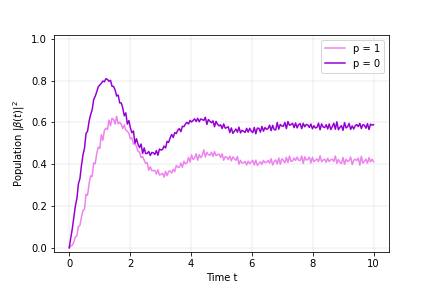
\includegraphics[width=\textwidth]{tex/figures/exercise07_02.png}
        \caption{Population $\abs{\beta}^2$ over time $t$ for $\gamma = 0.01$ and $p = 0.095$ and $0.05$. A lower $p$ corresponds to a higher thermal excitation rate and higher asymptote.}
        \label{fig:exercise07_02}
    \end{subfigure}
    \begin{subfigure}[t]{0.48\textwidth}
        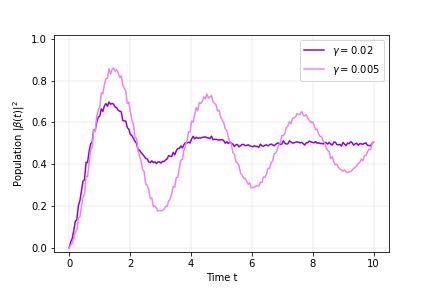
\includegraphics[width=\textwidth]{tex/figures/exercise07_03.png}
        \caption{Population $\abs{\beta}^2$ over time $t$ for $p = 0.5$ and $\gamma = 0.002$ and $0.005$. A higher $\gamma$ corresponds to a higher spontaneous emission rate and stronger dampening, which is clearly visible for $\gamma = 0.02$.}
        \label{fig:exercise07_03}
    \end{subfigure}
    \\
    \begin{subfigure}[b]{\textwidth}
        \centering
        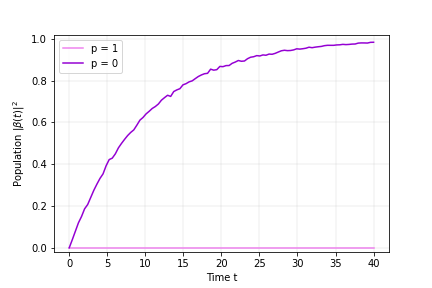
\includegraphics[width=0.48\textwidth]{tex/figures/exercise07_04.png}
        \caption{Population $\abs{\beta}^2$ over time $t$ for $\gamma = 0.02$ and $p = 1$ and $0$, without a driving term. At $p = 0$ GAD is an amplitude enhancing channel, that eventually turns all initial states to $\ket{1}$. With $p = 1$ GAD equals to the normal dampening channel, where all initial states end up in $\ket{0}$.}
        \label{fig:exercise07_04}
    \end{subfigure}
\end{figure}

\section{Single-Qubit Tomography}
Quantum state tomography is the method for reconstructing a qubit state by measuring the expectation values of the Pauli operators $\hat{\sigma}_i$. One can reconstruct the qubit state from these expectation values because the Pauli operators form an orthonormal basis of the $2\times2$ Hilbert space. Thus every qubit density matrix $\rho$ can be expressed as
\begin{equation}
    \rho = \Vec{c} \cdot \Vec{\hat{\sigma}}
\end{equation}
with $\Vec{\hat{\sigma}} = \{\mathbb{1}, \sigmax,\sigmay, \sigmaz\}$ the pseudo-vector of Pauli matrices and the vector coefficients  $\vec{c} = \frac{1}{2}\langle\Vec{\hat{\sigma}}\rangle$. Measuring the identity matrix contribution is not necessary since it's defined by the normalization condition $\operatorname{Tr}(\rho) =1 \rightarrow c_0 = \frac{1}{2}$. 

Usually the measurement basis for a quantum system is the z-basis. To measure $\langle\sigmax\rangle$ and $\langle\sigmay\rangle$ we need to perform a basis transformation from the measurement basis to the desired one using the cirq native gate set.
\subsubsection{Exercise 8}
The basis transformations for measurements in the x- and y-basis are
\begin{equation}
\yx{HZH} = \frac{1}{\sqrt{2}}\begin{pmatrix} 1&1\\1&1\end{pmatrix} \begin{pmatrix} 1&0\\0&-1\end{pmatrix}  \frac{1}{\sqrt{2}}\begin{pmatrix} 1&1\\1&1\end{pmatrix}  = \begin{pmatrix} 0&1\\1&0\end{pmatrix} = \yx{X} ,
\end{equation}
\begin{equation}
    \yx{SHZHS^\dagger} = \begin{pmatrix} 1&0\\0&i\end{pmatrix}\hadamard \begin{pmatrix} 1&0\\0&-1\end{pmatrix} \hadamard \begin{pmatrix} 1&0\\0&-i\end{pmatrix} = \begin{pmatrix} 0&-i\\i&0\end{pmatrix} = \yx{Y}.
\end{equation}
We demonstrate the quantum state tomography using cirq by simulating the measurement of the coefficient vector $\vec{c}$ and reconstructing the density matrix for the state $\ket{\Psi} = TH\ket{0} = \frac{1}{\sqrt{2}} \left(\ket{0} + e^{i\frac{\pi}{4}}\ket{1}\right)$. The measurements yield 
\begin{equation}
\vec{c} = \frac{1}{2}\begin{pmatrix}1\\0.000976\\0.706706\\0.706706\end{pmatrix}
\end{equation}
for the coefficients and thus for the reconstructed density matrix:
\begin{equation}
    \rho = \begin{pmatrix}0.500488 & 0.353353-0.353353\iu \\0.353353+0.353353\iu & 0.499512\end{pmatrix}
\end{equation}
To extract the qubit state from this density we must simply remind ourselves that an arbitrary desinty matrix for a pure qubit state is given by 

\begin{equation}
\rho = \begin{pmatrix} \abs{\alpha^2}& \alpha\beta^*\\\alpha^*\beta& \abs{\beta^2} \end{pmatrix}.
\end{equation}
We can therefore simply read-off the qubit state to be: $\ket{\Psi}_{tomo} = 0.70745196 \ket{0} + (0.4997558 +0.4997558\iu) \ket{1}$. We can thus see that the single-qubit tomography method reconstructs $\ket{\Psi}$ very well.

Equipped with this knowledge, we can now confidently use this method to reconstruct the oscillating qubit state from the Rabi oscillation. Figure \ref{fig:tomo} shows the population of the $\ket{1}$ state calculated using the analytical solution from equation \eqref{eq:population1} and using single-qubit tomography. As expected, the tomography reconstruction agrees well with the analytical solution.

\begin{figure}[h]
    \centering
    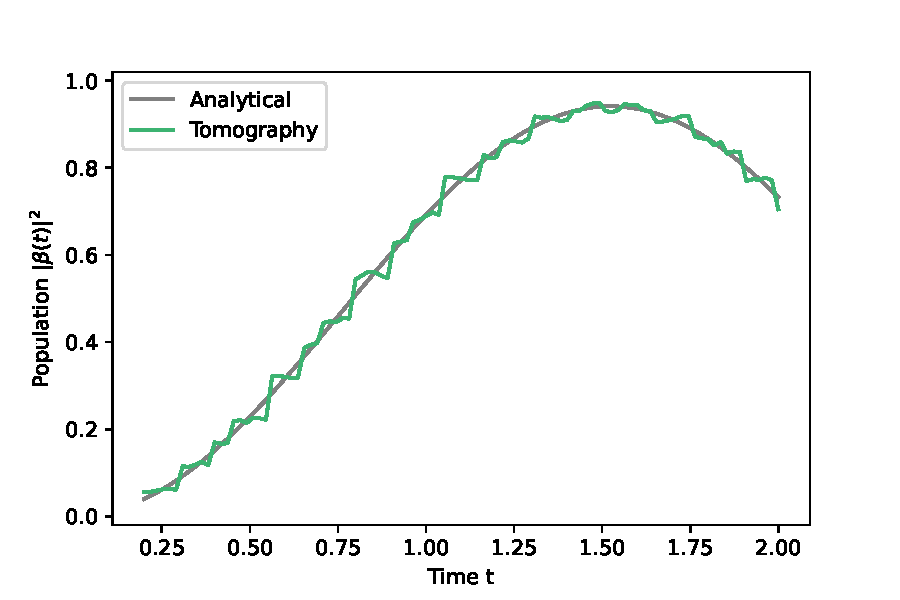
\includegraphics[width = 0.7\textwidth]{tex/figures/exercise10.pdf}
    \caption{Population $\abs{\beta}^2$ over time $t$ during a Rabi oscillation. State calculated using the analytical equation \eqref{eq:population1} and the state tomography sequence.}
    \label{fig:tomo}
\end{figure}

\section{Variational Quantum Eigensolver}
The variational quantum eigensolver (VQE) is a hybrid
quantum-classical algorithm that makes use of the variational method to find eigenvalues of a Hamiltonian. Let us consider a two-qubit cluster state Hamiltonian:
\begin{equation}
    \hat{H} = -\sigmax^1\sigmaz^2 - \sigmaz^1\sigmax^2
    \label{eq:HamVQE}
\end{equation} There are two main steps to applying the VQE algorithm. 

First, we construct a parameterized circuit ansatz, as seen in figure \ref{fig:variational_ansatz} which prepares the trial state: 
\begin{equation}
    \label{eq:trialstate}
    \ket{\psi(a, b)} = \exp\left[\mathrm{i}a \left(\sigmaz^1+\sigmaz^2\right)\right] \exp\left[\mathrm{i}b\left(\sigmax^1\sigmaz^2 + \sigmaz^1\sigmax^2\right)\right] \ket{00}
\end{equation}
To do so we define the two two-qubit gates $\mathrm{RZX} = \exp\left(\mathrm{i}b\left(\sigmaz \otimes \sigmax\right)\right)$ and $\mathrm{RXZ} = \exp\left(\mathrm{i}b\left(\sigmax \otimes \sigmaz\right)\right)$. 

\begin{figure}[h]
    \centering
    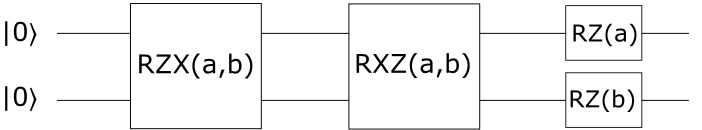
\includegraphics[width=0.6\linewidth]{tex/figures/CircuitEx10.png}
    \caption{Quantum circuit for creating the parameterized trial state from equation \eqref{eq:trialstate}}
    \label{fig:variational_ansatz}
\end{figure}

To find the minimum energy state, we make use of a simple grid search over the whole parameter space for a and b. For each choice a and b, we measure the energy expectation value and plot the results on a heat map to find the best trial state. 

\begin{figure}[h]
    \centering
    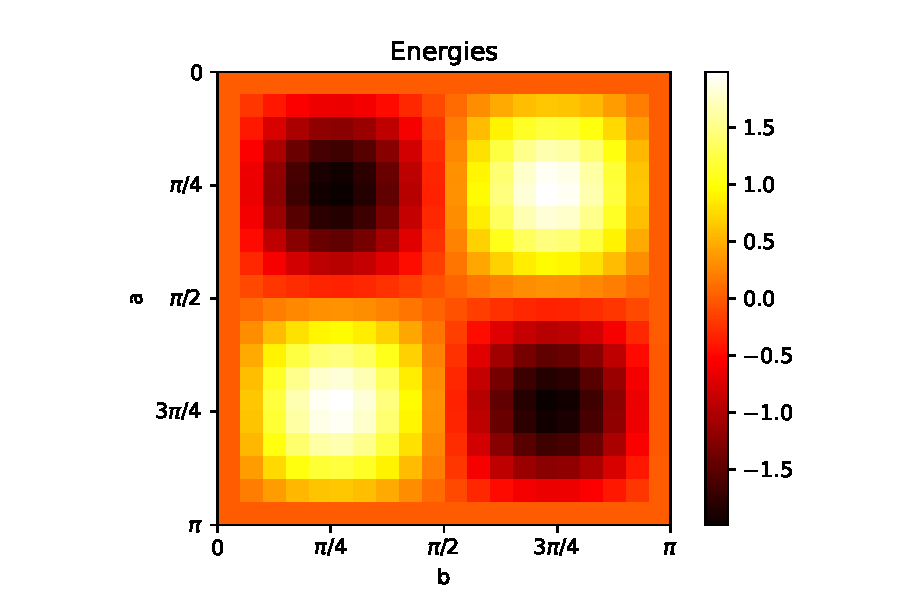
\includegraphics[width=0.8\linewidth]{tex/figures/exercise12.pdf}
    \caption{Energy expectation value for the Hamiltonian \eqref{eq:HamVQE} as a function of the trial state parameters a and b defined in \eqref{eq:trialstate}.}
    \label{fig:heatmap1}
\end{figure}

Using the best trial state, we find an approximate ground state energy of $E_0 = -1.986$.

To benchmark the approximate solution, we compare it to the exact solution of the ground state:
\begin{equation}
    \ket{\mathrm{\psi}} = \frac{1}{\sqrt{2}} \left(\ket{1-} + \ket{0+} \right)
\end{equation}
\begin{equation}
    \hat{H}\ket{\psi} = \left(-\sigmax^1\sigmaz^2 - \sigmaz^1\sigmax^2 \right) \left(\frac{1}{\sqrt{2}} \left(\ket{1-} + \ket{0+} \right)\right) = -2\ket{\psi}
\end{equation}

So we see that the approximation agrees well with the exact solution of $E_0 = -2$.

Lastly, we compute a landscape for the bipartition entanglement entropy over the parameter grid, see heat map \ref{fig:Ex15}, and compare it to the energy landscape. The first thing one notes is that, unlike the energy landscape, the entanglement entropy is independent of $a$ (within numerical accuracy). This is to be expected, since the rotations that depend on $a$ are local unitaries which cannot influence entanglement. The second thing one notices is that areas with high absolute energy value correspond to areas of high entanglement entropy except when $a\approx\frac{\pi}{2}$, in which case $a$ introduces a relative phase between the terms such that the energy vanishes.
\begin{figure}
    \centering
    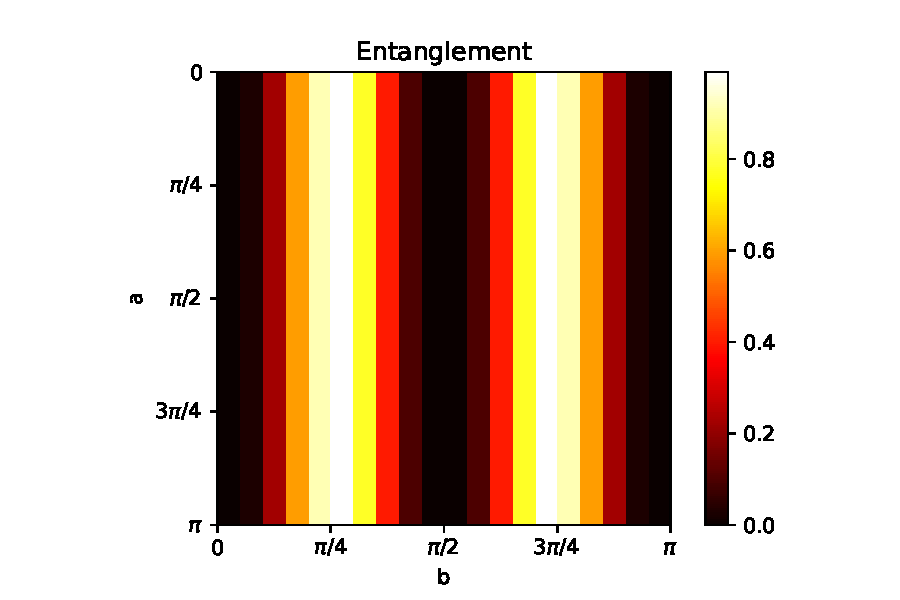
\includegraphics[width = 0.8\textwidth]{tex/figures/exercise15.pdf}
    \caption{Bipartition entanglement entropy of the trial state from equation \eqref{eq:trialstate} as a function of the parameters $a$ and $b$.}
    \label{fig:Ex15}
\end{figure}

    \chapter{Day 2 -- Time Evolution}
    \section{Dynamical Quantum Phase Transitions}
Dynamical quantum phase transitions (DQPT) are non-equilibrium phase transitions in quantum many-body systems that occour on transient time scales and are driven by progressing time as opposed to conventional phase transitions, which are driven by parameters such as temperature or pressure. 

At the phase transition certain physical quantities become non-analytic as a function of time. We begin by taking a closer look at the relevant physical quantities.

For more conventional equilibrium phase transitions the central object is the partition function
\begin{equation}
    \label{eq:partition}
    Z = \yx{Tr}\left(\exp\left(-\beta\hat{H}(\alpha)\right)\right)= \exp\left(-\beta Nf(\beta,\alpha)\right)
\end{equation}
with the inverse of the temperature $\beta=\frac{1}{T}$, a Hamiltonian $\hat{H}$ that depends on a set of parameters $\alpha$, the system size $N$ and the free energy density $f(\alpha,\beta)$. If $f(\alpha,\beta)$ becomes non-analytic as a function of the parameters $\alpha$ and at zero-temperature, one speaks of a quantum phase transition. For dynamical phase transitions we define quantities that are formally similiar to the partition function. Consider a many-body system with Hamiltonian $H_0$ in its ground state $\Psi_0$. In a process called quantum quench the Hamiltonian is changed nearly instantaneously to $H$ at $t = 0$. Following the quench the state will evolve according to the Schroedinger equation with $\ket{\Psi_0(t)} = e^{-i\hat{H}t}\ket{\Psi_0}$. The amplitude and probability to return to the ground state at time $t$ are then termed Loschmidt amplitude and Loschmidt echo
\begin{align}
    \mathcal{G}(t) &= \bra{\Psi_0}e^{-i\hat{H}t}\ket{\Psi_0}, \\
    \mathcal{L}(t) &= \left|\bra{\Psi_0}\ket{\Psi_0(t)}\right|^2 .
\end{align}
The Loschmidt echo has an exponential dependence on system size $N$, revealing the formal similarity to the partition function \eqref{eq:partition} after defining the Loschmidt rate $\lambda(t)$ through
\begin{equation}
    \mathcal{L} = e^{-N\lambda(t)}.
\end{equation}
The DQPTs will show up as non-analytical points in the Loschmidt rate, in analogy with critical points in the equilibrium phase transitions.
\subsubsection{Exercise 1}
The rate function $g(t)$ in $\mathcal{G}(t) = e^{-Ng(t)}$ is connected to the Loschmidt rate with $\lambda(t) = 2\Re{[g(t)]}$, following directly from the definitions
\begin{equation}
    \mathcal{L}(t) = \abs{\mathcal{G}(t)}^2 = e^{-Ng(t)}e^{-Ng^*(t)} = e^{-2N\Re{[g(t)]}} = e^{-N\lambda(t)}.
\end{equation}
For systems with $N_\mathrm{gs}$ degenerate ground states $\Psi_i$ the Loschmidt echo is the probability to return to any of the ground states and therefore sums over all return probalities
\begin{equation}
    \mathcal{L}(t) = \sum^{N_\mathrm{gs}-1}_{i=0}\left|\bra{\Psi_i}\ket{\Psi_0(t)}\right|^2.
\end{equation}
The total Loschmidt rate $\lambda(t)$ is still extracted by taking the logarithm $\lambda(t) = - \frac{1}{N}\ln\mathcal{L}(t)$, however, the additional ground states allow us to introduce individual rates $\lambda_i(t)$
\begin{equation}
    e^{-N\lambda_i(t)} = \left|\bra{\Psi_i}\ket{\Psi_0(t)}\right|^2.
\end{equation}
\subsubsection{Exercise 2}
In the thermodynamic limit $N \to \infty$ the total Loschmidt rate $\lambda(t)$ becomes the smallest individual rate $\lambda(t) = \operatorname{min}[\lambda_i(t)]$. This equality is shown by factoring out the term $e^{-N\lambda_\mathrm{min}}$ in the Loschmidt definition, ensuring that all remaining exponential terms have a negative argument $-N(\lambda_i - \lambda_\mathrm{min}) < 0$. Then the product formula $\ln a\cdot b = \ln a + \ln b$ is applied.
\begin{equation*}
    \lambda(t) = - \lim_{N\to\infty}\frac{1}{N}\ln \sum^{N_\mathrm{gs}-1}_{i=0}e^{-N\lambda_i} = - \lim_{N\to\infty}\frac{1}{N}\ln \left[e^{-N\lambda_\mathrm{min}}\sum^{N_\mathrm{gs}-1}_{i=0}e^{-N(\lambda_i-\lambda_\mathrm{min})}\right]
\end{equation*}
 All of the terms, except the minimum rate, vanish in the limit after using $\ln 1 + x \simeq x$ for $x \ll 1$.
 \begin{equation*}
    \lambda(t) = \lambda_\mathrm{min} - \lim_{N\to\infty}\frac{1}{N}\ln\left[1 + \sum^{N_\mathrm{gs}-1}_{i=\neq\mathrm{min}}e^{-N(\lambda_i-\lambda_\mathrm{min})}\right] \simeq \lambda_\mathrm{min} + \lim_{N\to\infty} \sum^{N_\mathrm{gs}-1}_{i=\neq\mathrm{min}} e^{-N(\lambda_i - \lambda_\mathrm{min})} = \lambda_\mathrm{min}
 \end{equation*}
\section{Transverse Field Ising Model}
The transverse field Ising model (TFI) describes a linear chain of $N$ qubits with nearest neighbor interaction. Due to its known analytical solution it is a suitable system to test the performance of numerical simulations, including our state vector simulation with trotterization. The TFI Hamiltonian $\hat{H}$ reads
\begin{equation}
    \label{eq:tfi}
    \hat{H} = -\frac{1}{2}\sum_{\left<i,j\right>}Z_iZ_j - \frac{g}{2}\sum_iX_i
\end{equation}
with $g$ being the strength of the transverse field. The $Z_iZ_j$ interaction strength is constant at unity. The system is symmetric under the parity operator 
\begin{equation}
    \hat{P} = \bigotimes_i X_i
\end{equation}
with spectrum $\{-1, 1\}$, since the commutator $[\hat{H}, \hat{P}] = 0$ vanishes. This is derived using the identities $X^2_i = \mathbb{1}$, $\hat{P} = \hat{P}^\dagger$ and $X_iZ_iX_i = -Z_i$. Each interaction term consists of two $Z_i$ matrices. This cancels out the negative sign when using the latter identity in computing $\hat{P}\hat{H}$.
\subsubsection{Exercise 3}
\begin{equation}
    \left[\hat{H}\hat{P} - \hat{P}\hat{H}\right]\hat{P}^\dagger = \hat{H} - \hat{P}\hat{H}\hat{P}^\dagger = \hat{H} - \hat{H} = 0 \Rightarrow [\hat{H}, \hat{P}] = 0
\end{equation}
In the limit $g = 0$ the ground states of $\hat{H}$ are $\ket{\Psi_0} = \ket{0\ldots 0}$ and $\ket{\Psi_1} = \ket{1\ldots1}$, while for $g \to \infty$ only one ground state $\ket{\Psi_+} = \ket{+\ldots+}$ exists. The magnetization of the system is the average spin orientation
\begin{equation}
    m_z = \frac{1}{N}\sum_i Z_i.
\end{equation}
For the ground states above it takes the values $m^0_z = \bra{\Psi_0}\frac{1}{N}\sum_i Z_i\ket{\Psi_0} = -1$, $m^1_z = +1$ and $m^+_z = 0$. $\ket{\Psi_+}$ has parity symmetry but no magnetization, while the states $\Psi_0$ and $\Psi_1$ have no parity symmetry but finite magnetization. This indicates a symmetry-broken ferromagnetic phase with $m_z \neq 0$ for some critical field strength $g_c$. To find the critical point the Hamiltonian is reexpressed with a new set of Ising variables
\begin{equation}
    \label{eq:ising}
    \tilde{Z_n} = \bigotimes_{i \leq n} X_i \quad \tilde{X_n} = Z_nZ_{n+1}
\end{equation}
to expose its self-dual structure. For identical behavior these variables need to share the same anticommutation relation $\{Z_i, X_i\} = 0$ as the original variables. Note that $\{Z_i, X_j\} = 0$ for any $i$ and $j$, as the operators act on different qubits. 
\subsubsection{Exercise 4}
The new anticommutator $\{\tilde{Z}_i, \tilde{X}_i\}$ is evaluated by factoring out the old anticommutator
\begin{equation}
    \left\{\tilde{Z_n}, \tilde{X_n}\right\} = \bigotimes_{i \leq n}X_iZ_nZ_{n+1} + Z_nZ_{n+1}\bigotimes_{i \leq n}X_i = \left[X_nZ_n + Z_nX_n\right]Z_{n+1}\bigotimes_{i \leq n-1}X_i = 0.
\end{equation}
The Hamiltonian $H$ now has the two forms where the second form can be rescaled to $\hat{\tilde{H}}$ through division with with $g$.
\begin{align}
    \hat{H} &= -\frac{1}{2}\sum^{N}_{i=1}Z_iZ_{i+1} - \frac{g}{2}\sum^N_{i=1}X_i\\
    &= - \frac{1}{2}\sum^{N}_{n=1}\tilde{X}_n - \frac{g}{2}\sum^{N}_{n=1}\tilde{Z}_n\tilde{Z}_{n+1} \\
    \hat{\tilde{H}} &= - \frac{1}{2}\sum^{N}_{n=1}\tilde{Z}_n\tilde{Z}_{n+1} - \frac{1}{2g}\sum^{N}_{n=1}\tilde{X}_n 
\end{align}
Multiplying a Hamiltonian does not change the dynamics of the system. The absolute energy scale is an arbitrary choice, therefore only the relative magnitude between the Hamiltonian terms is physical. Specifically, at the critical field value $g_c$ both Hamiltonians $\hat{H}$ and $\hat{\tilde{H}}$ predict the same phase transition. By comparison the critical field has to assume $g_c = \frac{1}{g_c} = 1$.
\subsubsection{Exercise 5}
The predictions for paramagnetic and ferromagnetic states in the TFI model have been made without considering any environment. For a canonical system at finite temperatures, the ferromagnetic order is not expected to survive over long ranges. In the 1D model the energy associated with a single domain wall is set by the $Z_iZ_{i+1}$ interaction term.
\begin{equation}
    \Delta E = - \frac{1}{2}\left<Z_iZ_{i+1}\right> = \frac{1}{2}
\end{equation}
In addition to the energy cost, every domain wall will add to the entropy $S$ of the chain. While the energy $E$ does not increase with system size $N$, the number of domain walls and the entropy does. For a system in contact with a thermal bath, the free energy $F = E - TS$ is minimized. The presence of many domain walls is therefore prefered due the higher entropy, despite the associated energy cost. This prevents ferromagnetic phases to extend over long distances.
\section{DQPTs in the TFI using Cirq}
In this section we study the time evolution generated by the Hamiltonian from equation \eqref{eq:tfi}.
\subsection{Implementing the time evolution}
As in day 1 of the FOPRA, we will perform a Trotter decomposition of the time evolution operator $\hat{U}(t)$. We may write 
\begin{equation}
U(t) = e^{-\iu\hat{H}t} = \left(e^{-\iu\hat{H}dt}\right)^{\frac{t}{dt}} = \left(e^{\hat{A}+\hat{B}}\right)^\frac{t}{dt}
\end{equation}
where $\hat{A} = -\frac{g}{2}dt \sum_i X_i$ and $\hat{B} = -\frac{1}{2}dt \sum_{\expval{i,j}}Z_iZ_j$.
\subsubsection{Exercises 6 and 7}
To implement this unitary in Cirq we first create a circuit that represents the evolution of the system by a small time step $dt$ up to second order Trotterization. To benchmark our results, we simulate the time evolution and extract the magnetization $m_z(t)$ as a function of time for a system of $L=10$ at $g=2$, starting from an initial state $\ket{\psi_0} = \ket{0...0}$ of all spins down. As seen in figure \ref{fig:ex6d2} the trotterization with timestep $dt = 0.25$ agrees very well with the exact solution obtained through diagonalizing the Hamiltonian.
\begin{figure}[h]
    \centering
    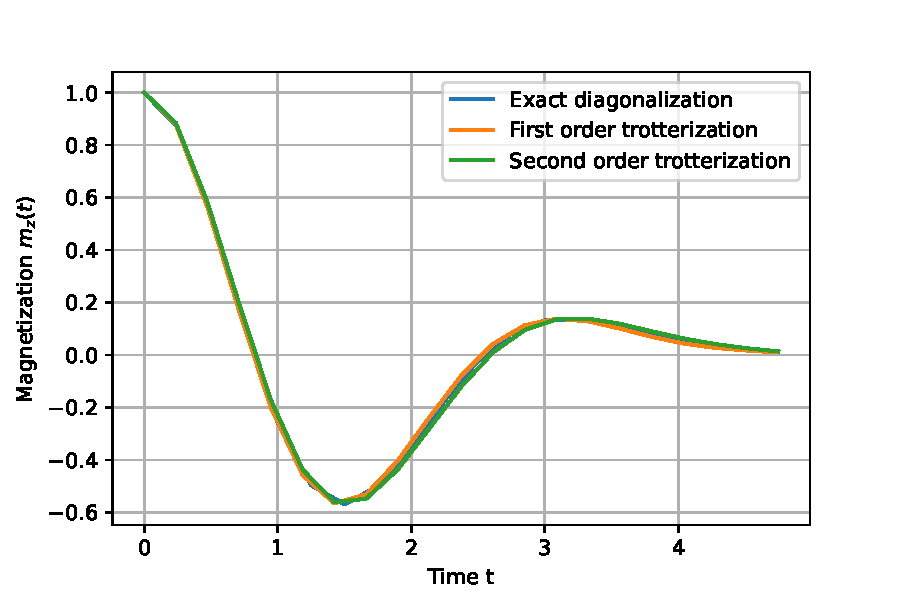
\includegraphics[width=0.6\textwidth]{tex/figures/Ex6d2.pdf}
    \caption{Magnetization $m_z$ over time $t$ for a $L = 10$ qubit chain in the tranverse field Ising model. First and second order trotterization delivers very accurate results compared to the exact evolution computed with diagonalization.}
    \label{fig:ex6d2}
\end{figure}

\subsubsection{Exercise 8}
We now want to evaluate the Loschmidt rate for an initial Hamiltonian $\hat{H}|_{g_0}$, where the two degenerate
ferromagnetic ground states are $\ket{\psi_0} =\ket{0...0}$ and $\ket{\psi_0} =\ket{1...1}$. Using the same time evolution as above, we extract the simulated Loschmidt rate by projecting back onto the ground state manifold. To study the results, we first plot the simulated Loschmidt rates for different system sizes while keeping the transverse field strength constant. We plot the results in figure \ref{fig:Loschmidt}. We can clearly see DQPTs occuring at $ts\approx1.8$ regardless of the system size.
\begin{figure}[h]
    \centering
    \caption{Simulated Loschmidt rates for different system sizes L with a strength of the transverse field g=2.}
    \label{fig:Loschmidt}
    \addtocounter{figure}{-1}
    \begin{subfigure}[t]{0.48\textwidth}
        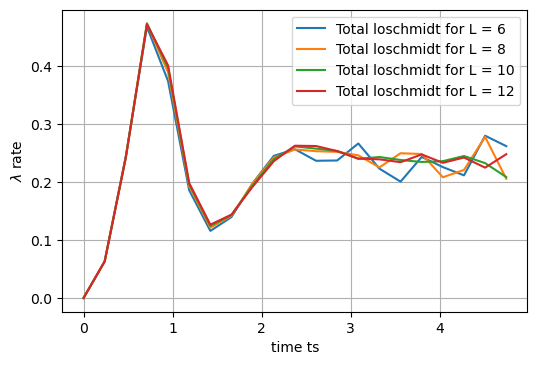
\includegraphics[width=\textwidth]{tex/figures/Lochschmidt.png}
        \caption{Loschmidt rate $\lambda(t)$}
    \end{subfigure}\\
    \begin{subfigure}[t]{0.48\textwidth}
        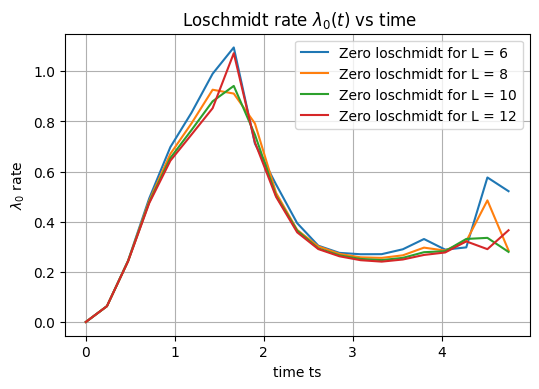
\includegraphics[width=\textwidth]{tex/figures/Loschmidt0.png}
         \caption{Loschmidt rate $\lambda_0(t)$}
    \end{subfigure}
    \begin{subfigure}[t]{0.48\textwidth}
        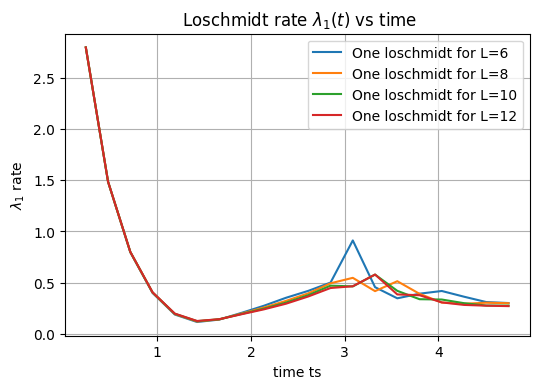
\includegraphics[width=\textwidth]{tex/figures/Loschmidt1.png}
         \caption{Loschmidt rate $\lambda_1(t)$}
    \end{subfigure}
\end{figure}

Next, in figure \ref{fig:LoschmidtManyGs} we do the same but keep the system size fixed and varying the transverse field strength. Again we can clearly see DQPTs occuring for $g>1$.

\begin{figure}[h]
    \centering
    \caption{Simulated Loschmidt rates for fixed sytsem size of L=12 and varying strength of the transverse field g=2.}
    \label{fig:LoschmidtManyGs}
    \addtocounter{figure}{-1}
    \begin{subfigure}[t]{0.48\textwidth}
        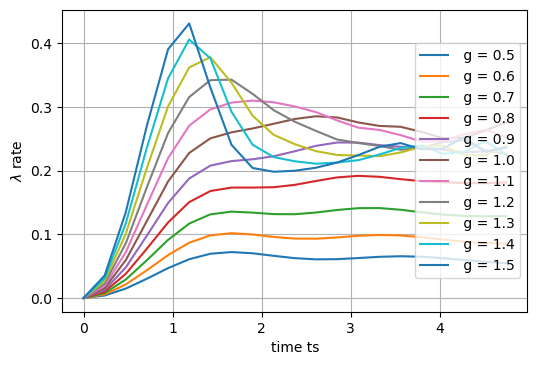
\includegraphics[width=\textwidth]{tex/figures/LochschmidtManyGs.png}
        \caption{Loschmidt rate $\lambda(t)$}
    \end{subfigure}\\
    \begin{subfigure}[t]{0.48\textwidth}
        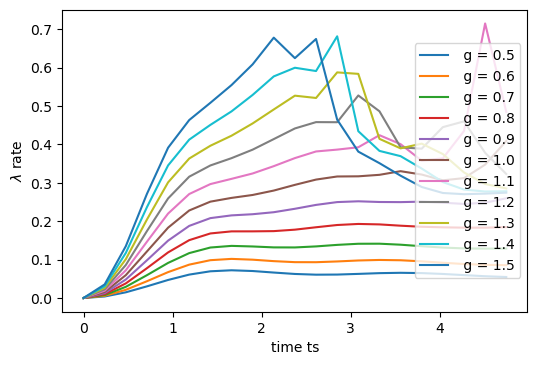
\includegraphics[width=\textwidth]{tex/figures/Lochschmidt0ManyGs.png}
         \caption{Loschmidt rate $\lambda_0(t)$}
    \end{subfigure}
    \begin{subfigure}[t]{0.48\textwidth}
        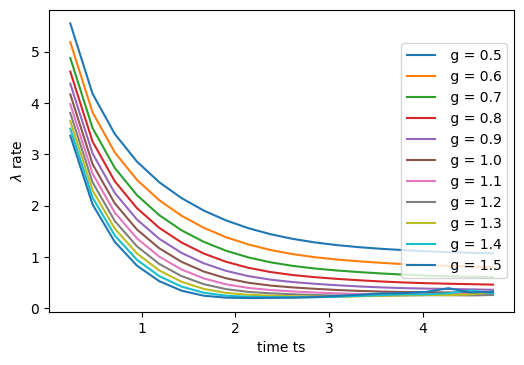
\includegraphics[width=\textwidth]{tex/figures/Lochschmidt1ManyGs.png}
         \caption{Loschmidt rate $\lambda_1(t)$}
    \end{subfigure}
\end{figure}

\subsubsection{Exercise 9}
Now we determine both the magnetization and Loschmidt echo as a function of time again, this time via repeated measurements. Figure \ref{fig:LoschMagComp} shows the results, which are essentially identical to the results from the exact solution. 
\begin{figure}[h!]
    \centering
    \caption{Loschmidt echo and magnetization as a function of time reconstructed using simulation of the exact solutions and using repeated measurements respectively.}
    \label{fig:LoschMagComp}
    \addtocounter{figure}{-1}
    \begin{subfigure}[t]{0.48\textwidth}
        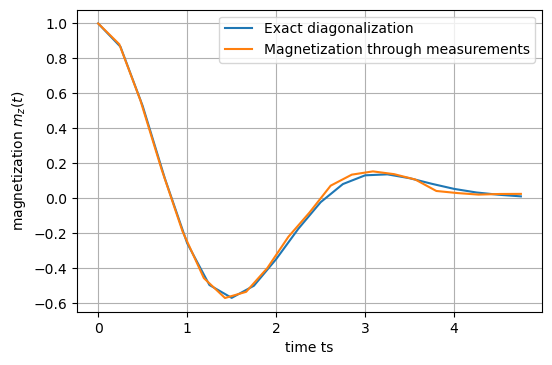
\includegraphics[width=\textwidth]{tex/figures/Magnetization2.png}
        \caption{Magnetization as a function of time.}
    \end{subfigure}
    \begin{subfigure}[t]{0.48\textwidth}
        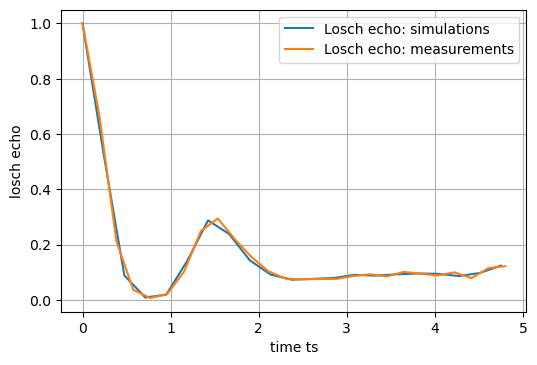
\includegraphics[width=\textwidth]{tex/figures/LoschEchoVSTime.png}
         \caption{Loschmidt echo as a function of time.}
    \end{subfigure}
\end{figure}

To determine how much sampling is in principle necessary to obtain accurate results, we notice that the maximum value of the total Loschmidt rate is approximately 0.5. Therefore,
\begin{equation}
    \frac{\min(\#\yx{of} \ket{0...0} \yx{or}\ket{1...1}}{\#\yx{of~samplings}} \approx \exp\left(-0.5N\right)
\end{equation}
In order to get accurate results, the expected frequency of getting the state $\ket{0...0}$ or $\ket{1..1}$must not be too small. In practice, we could set the expected frequency of ground state to be larger than 10, then the sampling times should fulfill.
\begin{equation}
    \#\yx{of~samplings} \geq 10\exp\left(-0.5N\right)
\end{equation}

\subsubsection{Exercise 10}
By putting both the magnetization and Loschmidt echo in the same plot, as seen in figure \ref{fig:MagAndLosch} we find that the turning point of magnetization (at around t = 1.5) corresponds to the second turning point of $\lambda(t)$.
\begin{figure}[h]
    \centering
    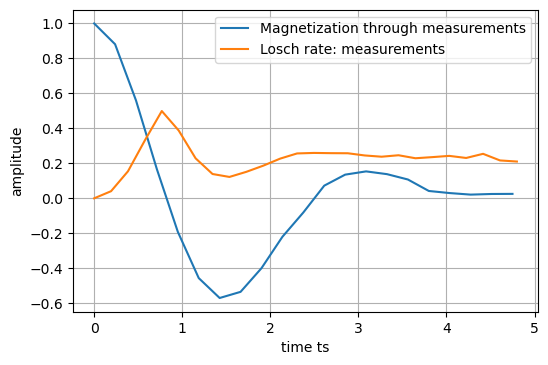
\includegraphics[width= 0.6\textwidth]{tex/figures/MagAndLosch.png}
    \caption{Magnetization and Loschmidt echo as a function of time.}
    \label{fig:MagAndLosch}
\end{figure}

\section{Tracking Entanglement Production}

After the quantum quench takes place, our state evolves from the initial product state to a system with higher entanglement. Due to this effect, it becomes increasingly harder to express the system using classical methods such as matrix product states (MPS).

In this exercise we will quantify the half-chain entanglement using the second Renyi entropy. The reduced density matrix of the subsystem $l$ in consideration is defined as:

\begin{equation}
    \rho_l = \Tr_r{[\rho]}
    \label{eq:reduced_matrix}
\end{equation}

Where the trace $\operatorname{Tr}_r$ is taken over the qubits that are not part of our subsystem, and $\rho$ is the matrix of the full system. Then, the second Renyi entropy is defined as \cite{manual}:

\begin{equation}
    S^{(2)} = - \log(\Tr{[\rho_l^2]})
    \label{eq:renyi_entropy}
\end{equation}


\subsubsection{Exercise 17}

From \cite{renyi_paper} we see there is an alternative way of obtaining the Renyi entropy through randomized measurements. First, we define the 1-qubit unitary gates from the circular unitary ensemble (CUE) acting on qubit $i$ defined as:

\begin{equation}
    \begin{split}
    U_i(a,b,c) & = \begin{pmatrix} e^{ia} \cos(b)  & e^{ic} \sin(b) \\ -e^{-ic} \sin(b) & e^{-ia} \cos(b) \end{pmatrix}. \\
     & = e^{i(a+c)Z/2} e^{ibY} e^{i(a-c)Z/2}
    \end{split}
\end{equation}

Where $a$ and $c$ are uniformly distributed over [$0$, $2\pi$], and $b$ is uniformly distributed over [0, $\pi/2$]\\

The second equality is useful for its code implementation. \textbf{Note: } This matrix differs by a minus sign from the one provided in the lab manual, since the gates proposed for cirq do not coincide.\\

The three parameters are sampled randomly generating a different $U_i$ to be applied on each of the qubits of the system. Then the subsystem is measured in the computational basis. From this, the probabilities $P_U(s_A)$ of measuring the bitstrings $s_A$ on the subsystem are obtained. With this information, an estimation of the purity ($\Tr{[\rho_l^2]}$) of the measured subsystem is obtained as:

\begin{equation}
    \label{eq:estimation_purity}
    X = 2^{L_a} \sum_{s_A, s^{'}_A} (-2)^{-D(s_A, s^{'}_A)} P_U(s_A) P_U(s^{'}_A)
\end{equation}

Where $D(s_A, s^{'}_A)$ represents the hamming distance between the bistrings $s_A$ and $s^{'}_A$, i.e. the number of different bits between the two bitstrings. \textbf{Important}: the sum runs over all possible tuples containing the combinations of bitstrings, this includes the cases where $s_A = s^{'}_A$ and symmetric cases such as $(s_A, s^{'}_A)$ and $(s^{'}_A, s_A)$. \\

This procedure is repeated for several independent realizations of the CUE unitaries, and the purity average $\overline{X}$ is used to obtain the final expression for the second Renyi entropy as:

\begin{equation}
    \label{eq:renyi_entropy_estimation}
    S^{(2)} = - \log(\overline{X})
\end{equation}

For its implementation in cirq, we write a function \texttt{U2\_CUE(qubit, symbs)} that applies the unitary $U_i$ from CUE to the qubit in the parameter \texttt{qubit}. The unitary is generated from the list of three parameters provided through \texttt{symbs}. Then, the hamming function defined above is also implemented in the code as \texttt{hamming(s1,s2)} where \texttt{s1} and \texttt{s2} are the two bitstrings to compare.\\

The time evolution of our system is studied under the trotterization from previous exercises using the simple evolution method and the Renyi entropy is calculated after each time step. For this simulation, we choose a total of 2000 measurement
repetitions, and 200 different instances of the CUE chosen using random generators over the correspondent ranges of the parameters.\\

The following graph shows the simulation for a hamiltonian using $g = 2$ applied on a two-qubit system that evolves  with a time step of $\delta t = 0.25$ for $N = \operatorname{int}(5/\delta t)$ time steps. For comparison, the exact value of the Renyi entropy was calculated through the density matrix of the total system after each time step provided by the function \texttt{cirq.Simulator().simulate}.

\begin{figure}[h]
    \label{fig:renyi_entropy}
    \centering
    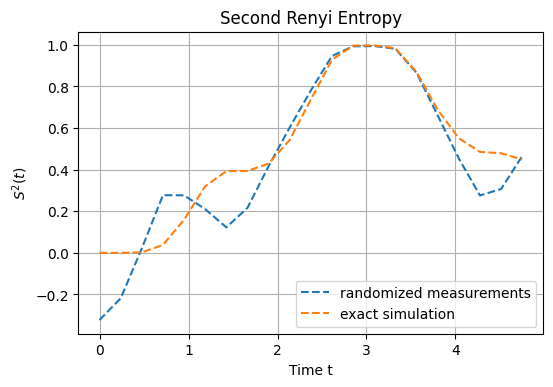
\includegraphics[width=0.8\textwidth]{tex/figures/exercise17.png}
    \caption{Second Renyi entropy simulation for a two-qubit system evolved by a first degree troterization}
\end{figure}

    \chapter{Conclusion}
    In this report, we used tensor networks methods to examine the behavior of 1D Ising chain Hamiltonian for medium-sized systems. In particular, these methods enabled the overcoming of the exponential scaling problem, which is common for numerical evaluation of quantum problems.\\
For the Ising chain, we were able to extract correlations between different sites, the magnetization and correlation length.

On day 2 we furthermore focused on the time evolution of the Ising model.
We were able to identify the excitation and therein connected kinks.
We therefore considered the time evolution of the correlations.
There one could nicely see the outwards propagation for no longitudinal field and the confinement for an applied longitudinal field.
We furthermore were able to show that our bound states are pretty close to the theoretical expectation - the negative roots of the Airy function.

    \newpage
\printbibliography

\end{document}